% !TEX program = pdflatex
% University of Malakand Thesis – Final version with official frontmatter
\documentclass[12pt, a4paper, oneside]{book}

\usepackage[utf8]{inputenc}
\usepackage[T1]{fontenc}
\usepackage{newtxtext,newtxmath}       % Times Roman text and math fonts
\makeatletter
\def\addfontfeatures#1{}
\def\fa@naming@exception#1#2#3{}
\makeatother
\renewcommand{\ttdefault}{lmtt}
\usepackage{geometry}
\usepackage{graphicx}
\usepackage[table]{xcolor}            % for rowcolors and cellcolor
\usepackage{setspace}
\usepackage{indentfirst}
\usepackage{fancyhdr}
\usepackage{titlesec}
\usepackage{caption}
\usepackage{enumitem}
\usepackage{multicol}
\usepackage{hyperref}
\usepackage{amsmath, amssymb}
\usepackage{booktabs}
\usepackage{tikz}
\usetikzlibrary{positioning,arrows.meta,shadows}
\usepackage{pgfplots}
\pgfplotsset{compat=1.18}
\usepackage{pgf-pie}
\usepackage{tcolorbox}
\tcbuselibrary{breakable,skins}
\usepackage{qrcode}
\usepackage{siunitx}
\usepackage{microtype}

% ===== MARGINS (as per University guidelines) =====
\geometry{
  a4paper,
  left=1.5in,
  right=1in,
  top=1in,
  bottom=1in,
  includeheadfoot
}

% ===== LINE SPACING 1.5 =====
\setstretch{1.5}

% ===== PAGE NUMBERING (bottom right, 0.75in from bottom) =====
\pagestyle{fancy}
\fancyhf{}
\setlength{\footskip}{0.75in}
\fancyfoot[R]{\thepage}
\renewcommand{\headrulewidth}{0pt}
\fancypagestyle{plain}{%
  \fancyhf{}%
  \fancyfoot[R]{\thepage}%
  \renewcommand{\headrulewidth}{0pt}%
}

% ===== SECTION NUMBERING (1, 1.1, 1.1.1) =====
\titleformat{\chapter}[display]
  {\normalfont\bfseries\centering}{\chaptertitlename\ \thechapter}{1em}{\Large}
\titlespacing*{\chapter}{0pt}{0pt}{30pt}
\titleformat{\section}
  {\normalfont\bfseries}{\thesection}{1em}{}
\titlespacing*{\section}{0pt}{14pt}{6pt}
\titleformat{\subsection}
  {\normalfont\bfseries}{\thesubsection}{1em}{}
\titlespacing*{\subsection}{0pt}{10pt}{4pt}

\captionsetup{font=small, labelfont=bf, justification=raggedright}

% ===== CUSTOM ENVIRONMENTS (from your original thesis) =====
\definecolor{Primary}{HTML}{1B2A3A}
\definecolor{Accent}{HTML}{3C78D8}
\definecolor{Light}{HTML}{F5F7FA}
\definecolor{Red}{HTML}{D62728}
\definecolor{Purple}{HTML}{9467BD}

\newtcolorbox{keyinsight}{
  enhanced, breakable, colback=Accent!5, colframe=Accent!50,
  leftrule=4pt, rightrule=0pt, toprule=0pt, bottomrule=0pt,
  arc=0pt, outer arc=0pt, left=10pt, right=10pt, top=6pt, bottom=6pt,
  before=\vspace{8pt}, after=\vspace{8pt}
}

\newtcolorbox{takeaway}{
  enhanced, breakable, colback=Accent!5, colframe=Accent!60,
  leftrule=4pt, rightrule=0pt, toprule=0pt, bottomrule=0pt,
  arc=4pt, outer arc=4pt, left=12pt, right=12pt, top=10pt, bottom=10pt,
  before=\vspace{12pt}, after=\vspace{12pt}, fontupper=\small
}

\setlist{nosep, leftmargin=*}

\hypersetup{
  colorlinks=true,
  linkcolor=black,
  citecolor=black,
  urlcolor=black
}

% ===== THESIS METADATA =====
\newcommand{\thesistitle}{Cardiovascular Disease Prediction Using Machine Learning}
\newcommand{\thesisauthorA}{Sajjad Alam}
\newcommand{\thesisauthorB}{Sajid Khan}
\newcommand{\thesisauthorC}{Ihsan Ullah}
\newcommand{\thesisdegree}{Bachelor of Science (Statistics)}
\newcommand{\thesisdept}{Department of Statistics}
\newcommand{\thesisuni}{University of Malakand}
\newcommand{\thesisyear}{2026}

\begin{document}
\onehalfspacing

% ============================================================
% FRONTMATTER – OFFICIAL FORMAT WITH TWO COVER PAGES
% ============================================================
\frontmatter

% ----- OUTER COVER PAGE (Annex-I style) -----
\begin{titlepage}
\thispagestyle{empty}
\centering
\vspace*{-0.5in}
{\fontsize{11pt}{13pt}\selectfont Annex-I\par}
\vspace{0.4in}

{\fontsize{14pt}{16pt}\selectfont \textbf{MPhil/PhD THESIS}\par}
{\fontsize{11pt}{13pt}\selectfont (Times New Roman, Bold and font size 14)\par}

\vspace{0.6in}

{\fontsize{16pt}{20pt}\selectfont \textbf{\MakeUppercase{\thesistitle}}\par}
{\fontsize{11pt}{13pt}\selectfont (times new roman, bold, capital and font size 16)\par}

\vspace{0.6in}

\begin{center}
  
\includegraphics[width=2.4in]{logo.png}   % replace with your logo file
\end{center}

\vspace{0.6in}

{\fontsize{14pt}{16pt}\selectfont \textbf{\MakeUppercase{\thesisauthorA}}\par}
{\fontsize{11pt}{13pt}\selectfont (times new roman, bold, capital and font size 14)\par}
\vspace{0.2in}
{\fontsize{14pt}{16pt}\selectfont \textbf{\MakeUppercase{\thesisauthorB}}\par}
\vspace{0.2in}
{\fontsize{14pt}{16pt}\selectfont \textbf{\MakeUppercase{\thesisauthorC}}\par}

\vfill

{\fontsize{16pt}{20pt}\selectfont \textbf{\thesisdept}\par}
\vspace{0.1in}
{\fontsize{16pt}{20pt}\selectfont \textbf{\thesisuni}\par}
\vspace{0.1in}
{\fontsize{16pt}{20pt}\selectfont \textbf{\thesisyear}\par}
\vspace{0.05in}
{\fontsize{11pt}{13pt}\selectfont (times new roman, bold, and font size 16)\par}
\end{titlepage}

% ----- INNER COVER PAGE -----
\newpage
\begin{titlepage}
\thispagestyle{empty}
\centering
\vspace*{-0.2in}

{\fontsize{16pt}{20pt}\selectfont \textbf{\MakeUppercase{\thesistitle}}\par}
{\fontsize{11pt}{13pt}\selectfont (times new roman, bold, capital and font size 16)\par}

\vspace{0.4in}

{\fontsize{12pt}{15pt}\selectfont A thesis submitted in partial fulfillment of the requirements for the degree of Master of Philosophy/PhD\par}
\vspace{0.05in}
{\fontsize{12pt}{15pt}\selectfont (Times New Roman and font size 12)\par}

\vspace{0.4in}

\begin{center}
  
\includegraphics[width=2.4in]{logo.png}
\end{center}

\vspace{0.3in}

{\fontsize{12pt}{15pt}\selectfont By\par}

\vspace{0.3in}

{\fontsize{14pt}{16pt}\selectfont \textbf{\MakeUppercase{\thesisauthorA}}\par}
\vspace{0.1in}
{\fontsize{14pt}{16pt}\selectfont \textbf{\MakeUppercase{\thesisauthorB}}\par}
\vspace{0.1in}
{\fontsize{14pt}{16pt}\selectfont \textbf{\MakeUppercase{\thesisauthorC}}\par}
{\fontsize{11pt}{13pt}\selectfont (times new roman, bold, capital and font size 14)\par}

\vfill

{\fontsize{14pt}{18pt}\selectfont \textbf{\thesisdept}\par}
\vspace{0.1in}
{\fontsize{14pt}{18pt}\selectfont \textbf{\thesisuni}\par}
\vspace{0.1in}
{\fontsize{14pt}{18pt}\selectfont \textbf{\thesisyear}\par}
\vspace{0.05in}
{\fontsize{11pt}{13pt}\selectfont (times new roman, bold, capital and font size 14)\par}
\end{titlepage}

% ----- PAGE NUMBERING STARTS WITH SMALL ROMAN ii -----
\pagenumbering{roman}
\setcounter{page}{2}

% ----- DECLARATION (three authors) -----
\clearpage
\thispagestyle{plain}
\vspace*{0.5cm}
\begin{center}
{\fontsize{14pt}{16pt}\selectfont \textbf{Declaration}\par}
\end{center}
\vspace{0.4in}

\noindent I, \textbf{\thesisauthorA}, \textbf{\thesisauthorB}, and \textbf{\thesisauthorC}, hereby declare that my MPhil/PhD thesis titled \textbf{``\thesistitle''} is my own work and has not been submitted previously by me for taking any other degree or professional qualification from \textbf{\thesisuni, Pakistan} or anywhere else in the country/world.

\noindent At any time if my statement is found to be incorrect even after my graduation, the university has the right to withdraw my Ph.D. degree.

\vspace{1.2in}

\noindent \textbf{\thesisauthorA}\\
Signature: \hrulefill \quad Date: \hrulefill

\vspace{0.3in}
\noindent \textbf{\thesisauthorB}\\
Signature: \hrulefill \quad Date: \hrulefill

\vspace{0.3in}
\noindent \textbf{\thesisauthorC}\\
Signature: \hrulefill \quad Date: \hrulefill

% ----- PLAGIARISM UNDERTAKING -----
\clearpage
\thispagestyle{plain}
\vspace*{0.5cm}
\begin{center}
{\fontsize{14pt}{16pt}\selectfont \textbf{Plagiarism Undertaking}\par}
\end{center}
\vspace{0.4in}

\noindent I solemnly declare that the research work presented in the thesis titled \textbf{``\thesistitle''} is solely my research work with no significant contribution from any other person. Small contribution/help wherever taken has been duly acknowledged and that complete thesis has been written by me.

\noindent I understand the zero-tolerance policy of the HEC and \textbf{\thesisuni, Pakistan} towards plagiarism. Therefore, I as an author of the above-titled thesis declare that no portion of my thesis has been plagiarized and any material used as a reference is properly referred/cited.

\noindent I undertake that if I am found guilty of any formal plagiarism in the above-titled thesis even after the award of PhD degree, the University reserves the right to withdraw/revoke my PhD degree, and that HEC and the University have the right to publish my name on the HEC/University Website on which names of students are placed who submitted plagiarized thesis.

\vspace{1.2in}

\noindent \textbf{\thesisauthorA}\\
Signature: \hrulefill \quad Date: \hrulefill

\vspace{0.3in}
\noindent \textbf{\thesisauthorB}\\
Signature: \hrulefill \quad Date: \hrulefill

\vspace{0.3in}
\noindent \textbf{\thesisauthorC}\\
Signature: \hrulefill \quad Date: \hrulefill

% ----- SUBMISSION AUTHORIZATION CERTIFICATE (for Evaluation) -----
\clearpage
\thispagestyle{plain}
\vspace*{0.5cm}
\begin{center}
{\fontsize{14pt}{16pt}\selectfont \textbf{Submission Authorization Certificate}\par}
\vspace{0.05in}
{\fontsize{11pt}{13pt}\selectfont (times new roman, bold, capital and font size 14)\par}
\vspace{0.2in}
{\fontsize{14pt}{16pt}\selectfont \textbf{(for Evaluation)}\par}
\end{center}
\vspace{0.4in}

\noindent Certified that the thesis of \textbf{\thesisauthorA, \thesisauthorB, \thesisauthorC} entitled, \textbf{``\thesistitle''} has been reviewed in the final form. Permission as indicated by the signatures given below is granted to submit the copies to \thesisuni\ for the final Evaluation Process.

\vspace{0.8in}

\noindent
\begin{tabular}{@{}p{0.45\textwidth}p{0.45\textwidth}@{}}
\textbf{Supervisor} & \textbf{Co-supervisor (if any)} \\
Signature: \hrulefill & Signature: \hrulefill \\
Name, Designation \& Affiliation: \hrulefill & Name, Designation \& Affiliation: \hrulefill
\end{tabular}

\vspace{0.6in}
\noindent \textbf{Chairman}\\
Signature: \hrulefill\\
Name, Designation \& Affiliation: \hrulefill

% ----- APPROVAL CERTIFICATE (for Award of Degree) -----
\clearpage
\thispagestyle{plain}
\vspace*{0.5cm}
\begin{center}
{\fontsize{14pt}{16pt}\selectfont \textbf{APPROVAL CERTIFICATE}\par}
\vspace{0.05in}
{\fontsize{11pt}{13pt}\selectfont (times new roman, bold, capital and font size 14)\par}
\vspace{0.2in}
{\fontsize{14pt}{16pt}\selectfont \textbf{(For the Award of Degree)}\par}
\end{center}
\vspace{0.4in}

\noindent It is certified that the work contained in this thesis entitled, \textbf{``\thesistitle''} was carried out by \textbf{\thesisauthorA, \thesisauthorB, \thesisauthorC} under my/our supervision. In my/our opinion, it is fully adequate, in scope and quality, for the degree of Master of Philosophy/Doctor of Philosophy in \textbf{Statistics}.

\vspace{0.6in}

\noindent \textbf{Approved by:}

\vspace{0.5in}

\noindent
\begin{tabular}{@{}p{0.45\textwidth}p{0.45\textwidth}@{}}
\rule{2.2in}{0.4pt} & \rule{2.2in}{0.4pt} \\
\textbf{Supervisor} & \textbf{Co-supervisor (if any)} \\
& \\
Name & Name \\
Designation and Affiliation & Designation and Affiliation
\end{tabular}

\vspace{0.6in}

\noindent \rule{2.2in}{0.4pt}\\
\textbf{External Examiner}\\
\\
Name\\
Designation and Affiliation

\vspace{0.6in}

\noindent \rule{2.2in}{0.4pt}\\
\textbf{Chairman}

% ----- DEDICATION -----
\clearpage
\thispagestyle{plain}
\chapter*{Dedication}
\addcontentsline{toc}{chapter}{Dedication}
\begin{center}
\emph{To our parents who always believed in us.}
\end{center}

% ----- ACKNOWLEDGMENTS -----
\clearpage
\thispagestyle{plain}
\chapter*{Acknowledgments}
\addcontentsline{toc}{chapter}{Acknowledgments}
We want to thank our supervisor for putting up with our questions. Also thanks to our teachers and our families. And of course the open‑source community – without them this would have been way harder.

% ----- TABLE OF CONTENTS -----
\clearpage
\phantomsection
\addcontentsline{toc}{chapter}{Contents}
\tableofcontents
\clearpage
\phantomsection
\addcontentsline{toc}{chapter}{List of Figures}
\listoffigures
\clearpage
\phantomsection
\addcontentsline{toc}{chapter}{List of Tables}
\listoftables

% ----- LIST OF ABBREVIATIONS -----
\clearpage
\thispagestyle{plain}
\chapter*{List of Abbreviations}
\addcontentsline{toc}{chapter}{List of Abbreviations}
\begin{multicols}{2}
\begin{itemize}
\item CVD: Cardiovascular disease
\item BMI: Body mass index
\item ROC: Receiver operating characteristic
\item AUC: Area under the curve
\item SHAP: SHapley Additive exPlanations
\item API: Application Programming Interface
\item ML: Machine Learning
\item SVM: Support Vector Machine
\item RF: Random Forest
\item XGB: XGBoost
\item LGBM: LightGBM
\end{itemize}
\end{multicols}

% ----- LIST OF PUBLICATIONS -----
\clearpage
\thispagestyle{plain}
\chapter*{List of Publications}
\addcontentsline{toc}{chapter}{List of Publications}
(If any)

% ----- ABSTRACT -----
\clearpage
\thispagestyle{plain}
\chapter*{Abstract}
\addcontentsline{toc}{chapter}{Abstract}
This thesis builds a working machine learning setup that predicts cardiovascular disease risk from everyday health measurements. We took a structured dataset with demographic info, clinical readings, and lifestyle habits then compared several models: Logistic Regression, SVM, Random Forest, a Neural Network, and gradient boosting (XGBoost/LightGBM). The best ones are served through a FastAPI backend with a simple web frontend. The system gives back a probability score, a yes/no decision based on a threshold, and SHAP explanations that show which factors pushed the prediction up or down.

% ============================================================
% MAINMATTER – YOUR FULL THESIS CONTENT (unchanged)
% ============================================================
\mainmatter
\pagenumbering{arabic}
\setcounter{page}{1}

% ================== CHAPTER 1 ==================
\chapter{INTRODUCTION}

\section{Background of the Study}

Cardiovascular disease. CVD for short. It's still one of the top causes of death around the world. Every year millions of people die from heart failure. Or coronary artery disease. Or stroke. That's what the WHO keeps telling us. I checked their reports. The numbers are insane.

These problems are usually tied to lifestyle. Eating badly. Not exercising. Smoking. Diabetes. High blood pressure. Being overweight. All that stuff. So yeah catching it early really matters. Like a lot. The earlier you find it the better the treatment can work. You can change your diet. Start medication. Exercise more. That's the whole idea.

I thought about this for a while. Why do so many people die from something we know about? Partly because they don't know they're at risk. Partly because doctors don't catch it early enough. That's where my project comes in.

Normally doctors diagnose based on their own experience. Lab tests. Clinical guidelines. That works fine most of the time. But sometimes it misses the subtle patterns hiding inside medical data. Like relationships that aren't obvious. A human can't look at a hundred variables at once. But a computer can.

Nowadays we have more healthcare data than ever. And computers are fast. So machine learning has become a good way to dig through large medical datasets. Help predict diseases. I mean that's exactly what I wanted to do.

Let me explain ML real quick. ML algorithms learn from past examples. Then they make predictions on new unseen data. In healthcare that means they can help doctors spot high-risk patients. Support early diagnosis. People have already used models like Logistic Regression. Random Forest. Support Vector Machines. Gradient Boosting. For all kinds of medical prediction tasks. I read a bunch of papers about it.

The dataset I used here includes a bunch of features. Age. Gender. Blood pressure. Cholesterol. Glucose. Smoking. Drinking. Physical activity. By looking at those features the ML models try to find patterns. Patterns that might signal whether someone is likely to get CVD. It's not magic. It's just math and data.

Using machine learning in healthcare could make diagnoses more accurate. Cut costs. Give doctors a second opinion. That's why building a reliable CVD prediction model is worth working on. And that's exactly what I did in this thesis. I built it. I tested it. I compared results.

\section{Problem Statement}

Medical science has improved a lot. No doubt. But heart disease still kills tons of people around the world. I looked at the statistics. It's depressing. Catching it early and stopping it before it gets bad -- that's really important. Everyone knows that.

The thing is traditional diagnosis mostly relies on doctors looking at clinical data by hand. They review test results. They check patient history. That takes a while. And honestly people mess up sometimes. Doctors get tired. They have too many patients. They miss stuff. That's just reality.

Medical datasets usually have a bunch of variables. Like ten or twenty or more. And all these complicated relationships between them. Some variables interact in weird ways. Old school statistical models just can't pick up the nonlinear patterns hidden in the risk factors. Linear regression for example. It assumes straight lines. But real health data isn't straight.

So yeah we really need smart systems. Systems that can dig through large amounts of medical data. And give us accurate predictions about heart disease risk. Without taking forever. Without making human errors.

Machine learning learns how to identify patterns in data without being explicitly coded to look for those patterns. That's the cool part. You just feed it data. It figures things out. This is great because many of the traditional approaches become too hard to use when the data isn't linear. Like when age and blood pressure don't have a simple relationship.

But here's the problem. Matching the right ML algorithm to the data isn't simple. It often feels like chasing shadows. You try one model. It does okay. You try another. It does better. You try a third. It does worse. There's no clear winner from the start.

It demands trial and testing and real-world checks before you're confident it works. You can't just guess. You have to actually run the experiments. That's what I did.

So what I wanted to do was create and train a variety of machine learning models on the same clinical dataset. Then determine which one gives the most accurate prediction for heart disease risk. Through a thorough comparison. With no shortcuts. I documented everything.

Let me restate the problem one more time. CVD kills people. Early detection saves lives. Current methods are slow and error-prone. ML can help but we don't know which model is best for this specific dataset. That's the gap. That's what my study tries to fill.

\section{Research Objectives}

I had a main goal. Simple one. Build an ML model that can predict CVD risk accurately. That's it. But I broke it down into smaller pieces. I needed a clear plan.

Let me list the specific things I wanted to achieve. I wrote these down before I started any coding.

\textbf{First objective.} Understand the dataset. I mean really look at it. Not just open it and run a model. I wanted to see the relationships between the medical attributes. Like how does age relate to blood pressure? Do smokers have higher cholesterol? I spent time on exploratory analysis. Made plots. Calculated correlations. Just got familiar with the data.

\textbf{Second objective.} Clean and prepare the data. Raw data is messy. Honestly. Missing values everywhere. Outliers that don't make sense. Different scales -- some features go from 0 to 1 but others go up to 300. I had to fix all that so the models could use it. I handled missing values. I capped outliers. I scaled the numerical features. I encoded categorical variables like gender and smoking. That took a while but it was worth it.

\textbf{Third objective.} Train several ML algorithms on the data. I didn't want to just try one model. That would be lazy. I picked a few common ones that people use in medical research. Logistic Regression because it's simple and interpretable. Random Forest because it handles non-linear stuff well. Support Vector Machine because it's good for classification with clear boundaries. Gradient Boosting because it often wins on tabular data. I trained each one on the same training set. Same random seed.

\textbf{Fourth objective.} Compare them using proper evaluation metrics. I couldn't just look at accuracy. Accuracy can lie. Especially if the classes are imbalanced -- like more healthy people than sick people. So I used multiple metrics. Precision. Recall. F1-score. ROC-AUC. Also confusion matrices. I wanted a fair comparison. Not just one number.

\textbf{Fifth objective.} Find out which features matter the most for prediction. This was important to me. I didn't just want a black box that spits out a number. I wanted to know why the model makes a decision. So I did feature importance analysis. For Random Forest it gives importance scores automatically. For others I used permutation importance. I found out which medical attributes are most helpful. Age? Blood pressure? Cholesterol? That knowledge could help doctors focus on the right risk factors.

So yeah those were my objectives. Five clear things. I followed each one step by step.

\section{Research Questions}

I tried to answer three main questions. Nothing fancy. Just the ones that matter.

\textbf{First question.} Can ML models correctly tell if a person has CVD using only clinical data? Like without expensive tests or specialist reviews. Just basic medical attributes. That would be useful in a lot of places.

\textbf{Second question.} Which algorithm works best on this dataset? Is it Logistic Regression? Random Forest? SVM? Gradient Boosting? I wanted a clear winner. Or at least a recommendation.

\textbf{Third question.} What are the most important risk factors? Which features drive the prediction the most? If we know that, maybe we can design better prevention programs.

That's it. Three questions. I answered them in Chapter 4.

\section{Significance of the Study}

This study shows that ML can help predict heart disease. I'm not the first to try it. But I did my own version. If it works well doctors could use it to catch high-risk patients early. Maybe prevent bad outcomes. Like heart attacks. Or strokes.

The model I built could be a decision support tool. Not replacing doctors. Just helping them. A doctor could enter a patient's data. The model gives a risk score. Then the doctor decides what to do. More tests. Lifestyle changes. Medication. That's the idea.

Also I hope this research encourages more people to try AI in healthcare. A lot of people are still skeptical. They think AI is complicated or unreliable. But my results show it can work. At least on this dataset.

Another thing. By identifying the most important features my study gives hints to doctors. Like focus on blood pressure. Focus on cholesterol. Those matter a lot. That's useful even without the full model.

So yeah. This isn't just for a grade. It could help real people someday.

\section{Scope of the Study}

I focused only on one structured dataset. It's a public dataset. I didn't collect it myself. I just used what was available.

I did all the usual steps. Preprocessing. Exploring the data. Training models. Evaluating them. Hyperparameter tuning too. I spent time on that.

But here's what I did not do. I did not deploy the model in a real hospital. That's a whole different thing. You need regulatory approval. Integration with electronic health records. Real-time data feeds. That's too much for a student thesis.

I also didn't use any other types of data. No medical images. No free-text clinical notes. Just numbers and categories. That's a limitation for sure.

And I only used one dataset. So my results might not generalize to other populations. Different countries. Different age groups. Different healthcare systems. Someone would need to test that.

So yeah. That's the scope. It's not everything. But it's a solid starting point.

\section{Structure of the Thesis}

Alright here's how the rest of the thesis is organized. Quick overview.

Chapter 2 is a literature review. I talk about what other people did. Their methods. Their results. Where my study fits in.

Chapter 3 explains my methods. The dataset. How I preprocessed it. Which ML algorithms I used. How I evaluated them. So someone else could replicate it.

Chapter 4 shows the results. Tables. Plots. Numbers. I compare each model. I show feature importance. I answer my research questions.

Chapter 5 wraps everything up. I summarize what I found. I talk about limitations. I give recommendations for future work.

That's the structure. Nothing crazy. Just standard thesis layout.

% ================== CHAPTER 2 ==================
\chapter{LITERATURE REVIEW}

\section{Introduction}
Lots of researchers have tried to predict CVD using ML. This chapter goes through some of that work. I look at common algorithms what datasets they used and what they found. Also I point out gaps that my study tries to fill.

\section{Cardiovascular Disease and Its Risk Factors}
First a quick reminder of what CVD is. It includes heart attacks strokes high blood pressure and other heart problems. Risk factors are things like age older people have higher risk gender men tend to get it earlier high blood pressure high cholesterol diabetes obesity smoking drinking too much alcohol and not moving enough. Some of these you can control like smoking some you can't like age. The WHO says lifestyle is a huge part of it.

\section{Machine Learning in Healthcare -- A Quick Overview}
ML is a branch of AI where computers learn from data without being explicitly programmed for every rule. In healthcare ML is used for diagnosis predicting patient outcomes analysing medical images even discovering new drugs. It's good at finding patterns that humans might miss. Common algorithms include logistic regression simple interpretable decision trees easy to explain random forests many trees together SVMs find a separating line/plane and neural networks deep learning. Each has pros and cons.

\section{Previous Studies on CVD Prediction}
A lot of papers exist. I'll mention a few.
One classic study by Detrano et al. (1989) used logistic regression and decision trees on the Cleveland heart disease dataset. Logistic regression gave a decent baseline. Decision trees helped understand which features mattered.
Another study used SVMs and random forests. They found that random forest an ensemble method performed better because it averages out the mistakes of many trees.
More recently gradient boosting methods like XGBoost and LightGBM have become popular. They build trees one after another each new tree trying to fix the errors of the previous ones. Many Kaggle competitions are won with these.
Neural networks deep learning have also been tried. They can model very complex relationships but need a lot of data and computing power. For medium-sized tabular datasets like the one I used gradient boosting often works just as well or better.

\section{Comparative Analysis of ML Algorithms}

Here is what I think about each algorithm's positive and negative aspects.

\begin{itemize}
\item \textbf{Logistic Regression:} It's simple. Fast. The results are easy to understand. So yeah that's nice. But here's the major drawback. It only models linear relationships. Real data isn't always linear. That's a problem.

\item \textbf{Decision Trees:} Visually they could be very appealing. You can draw them. That's cool. But at times they get confusing. Because they overfit. Honestly overfitting is a pain.

\item \textbf{Random Forest:} It's a group of decision trees. Very reliable. Mitigates overfitting a lot. I liked using this one.

\item \textbf{SVM:} Works fine in high dimensional spaces. That's good. But finding the right setting is not easy. You have to tweak a bunch of stuff. Takes time.

\item \textbf{Gradient Boosting (XGBoost, LightGBM)} Most of the time it's the best choice for tabular data. That's what I saw too. Works really well.

\item \textbf{Neural Networks:} Highly capable. But they require very precise tuning. And they're not very interpretable. You can't easily see why they made a prediction. That bothers me.
\end{itemize}
\section{Research Gap -- Why This Study is Needed}
From reading the literature I noticed that many studies either use only a couple of algorithms or work on small datasets. Also not many of them deploy the model as a web service or include explainability SHAP. So my study tries to do more: compare many models use a large public dataset and also build a working API with SHAP explanations.

\section{Summary of Literature Review}
There's a solid body of evidence that ML can predict CVD. Ensemble methods random forest gradient boosting tend to perform best. Still there is room for a more comprehensive comparison and a real-world demonstration the API. That's what I'll do next.

\begin{takeaway}
\textbf{Key points from Chapter 2:}
\begin{itemize}
  \item ML has been successfully applied to CVD prediction using various algorithms.
  \item Gradient boosting (XGBoost, LightGBM) often outperforms traditional methods.
  \item Few studies combine a thorough multi-model comparison with a deployable API and SHAP explanations.
  \item This work fills that gap by evaluating seven models and providing a web service with interpretability.
\end{itemize}
\end{takeaway}

% ================== CHAPTER 3 ==================
\chapter{RESEARCH METHODOLOGY}

\section{Introduction}
let's get into how I actually did the work. This chapter walks through everything step by step -- where the data came from, how I scrubbed it, what features I cooked up, the models I tried, and how I tested them. I'm gonna keep it real, no fluff. If something didn't work I'll say so. It's all about being clear so someone else can pick up my code and run with it.

When I first opened the CSV file I had this weird mix of excitement and panic. Seventy thousand rows of real medical data just sitting there waiting to be explored. But I knew that raw data is never ready for prime time. There's always something broken hiding in the columns, and if you don't catch it early your whole model becomes garbage in, garbage out. So I spent a lot of time just staring at the numbers, checking ranges, plotting histograms, and thinking about what could go wrong. I think it's the most underrated part of machine learning -- the boring cleanup phase that nobody writes papers about but that actually makes or breaks everything.

\section{Dataset Description}
I grabbed the Cardiovascular Disease dataset from Kaggle -- the one by sulianova. It's a public thing, no privacy issues. Original size was exactly 70,000 rows. After cleaning (mostly kicking out weird blood pressure readings) I ended up with 68,576 rows. That's still plenty of data to work with.

The dataset came with 12 columns. One column called `id` was just a row number so I dropped it immediately. Then there were 11 features and the target variable `cardio`. If `cardio` is 1, the person has heart disease; if it's 0, they don't. Simple enough. The features are a mix: some are continuous numbers, some are categories disguised as numbers, and some are just yes/no flags.

Here's what each feature means. I saved this list as a quick reference so I wouldn't forget while coding.

\textbf{age} -- originally in days, I divided by 365.25 to get years. That's more readable and it's what a doctor would use.

\textbf{gender} -- 1 for female, 2 for male. A bit old-school but fine.

\textbf{height} -- in centimeters. I would have preferred meters but whatever.

\textbf{weight} -- kilograms, which makes BMI calculation easy later.

\textbf{ap\_hi} -- systolic blood pressure, the ``top'' number.

\textbf{ap\_lo} -- diastolic blood pressure, the ``bottom'' number.

\textbf{cholesterol} -- three levels: 1 normal, 2 above normal, 3 well above normal. No actual mg/dL values, just categories.

\textbf{gluc} -- same three-level scale for glucose. Again, no real numbers, just levels.

\textbf{smoke} -- 1 if they smoke 0 if not. Self-reported so I took it with a grain of salt.

\textbf{alco} -- 1 if they drink alcohol, 0 if not. Same problem as smoking: people lie.

\textbf{active} -- 1 if they do regular physical activity. Who knows what ``regular'' means to each person.

One thing I noticed early on: cholesterol and gluc are ordinal categories, not real measurements. That's a bit limiting because you can't see subtle differences, only big jumps. But that's what the dataset gave me, so I worked with it.

\begin{keyinsight}
Data leakage. I made dead sure not to use any output column like `prediction` or `probability` as an input. Those only exist after the model runs -- if you feed them back in you get a fake perfect score. So I never even looked at them during training.
\end{keyinsight}

\section{Data Preprocessing -- Step by Step}
I didn't just throw raw data into a model. There were a bunch of grubby bits to handle first. I like to think of preprocessing as washing vegetables before cooking -- you don't skip it unless you want dirt in your soup.

\subsection{Handling Missing Values}
Honestly? The dataset had zero missing cells. I double-checked with `df.isnull().sum()` -- all zeros. No NaNs, no blanks. That's unusual for a Kaggle dataset but I'm not complaining. Still, I wrote a small function that replaces missing numeric values with the median and missing categorical ones with the mode. Just in case someone feeds in a dirty version later. Better safe than sorry.

\subsection{Data Cleaning}
Blood pressure values were the messiest. I found rows where ap\_hi was less than ap\_lo -- that's physically impossible unless you're measuring upside down. I also removed rows where systolic was over 250 mmHg or under 80, and diastolic under 40 or over 150. Those are either typos or extreme outliers that would mess up my models. In total I removed about 1,400 rows. That's only 2\% of the dataset, so no big loss.

I also checked height and weight. Some people had height like 55 cm or weight 200 kg. Could be data entry errors, could be real outliers. I decided not to drop them -- I'd rather keep the data and let BMI handle the combination. If someone is 55 cm tall and 200 kg, their BMI will be astronomical, and the model can learn from that. Plus, after cleaning blood pressure I felt I'd done enough cutting.

Age needed a quick conversion. The raw column was in days -- like 12000 days. I divided by 365.25 to get years. A few people came out above 100, but this is a Russian dataset and it's possible. I kept them. The histogram later showed most folks were middle-aged, which makes sense for a heart disease study.

\subsection{Feature Encoding}
All features were already numeric, so I didn't need one-hot encoding or label encoding. Gender is 1/2, cholesterol and gluc are 1/2/3, smoke/alco/active are 0/1. For tree-based models that's fine -- they can split on integers. For linear models and SVM, I scaled the continuous features. So I just kept the categories as raw numbers and let the models figure it out.

\subsection{Feature Scaling}
I used `StandardScaler` from scikit-learn on the continuous columns: age, height, weight, ap\_hi, ap\_lo. That transforms each column to mean 0 and standard deviation 1. It's important for distance-based models like SVM and neural nets, where big numbers like age (30--65) would dominate over smaller numbers like cholesterol (1--3). Trees don't care about scaling, but I scaled anyway so I could use the same preprocessed array for all models. The categorical-like ones -- cholesterol, gluc, smoke, alco, active -- were left untouched because they're already on a small scale and scaling them might destroy their meaning.

\subsection{Feature Engineering}
This was honestly the most fun part. I got to think like a doctor and create new features that combine the raw measurements into medical concepts. Here's what I made.

Pulse pressure is just $ap_{\text{hi}} - ap_{\text{lo}}$. A high pulse pressure can signal stiff arteries, which is a risk factor for heart disease. Mean arterial pressure, or MAP, is $\frac{2 \cdot ap_{\text{lo}} + ap_{\text{hi}}}{3}$. It's a better overall measure of perfusion than either number alone. I created a hypertension flag: 1 if $ap_{\text{hi}} > 140$ or $ap_{\text{lo}} > 90$, else 0. Straight from WHO guidelines. High cholesterol flag: 1 if cholesterol > 1. High glucose flag: 1 if gluc > 1. I binarised these because many risk scores just care about ``high'' vs ``normal'' -- the exact level might not add much beyond that. And finally, BMI: $\text{weight} / (\text{height}/100)^2$. Under 18.5 is underweight, 25+ overweight, 30+ obese.

After all this the feature set jumped from 11 to 16. Not a huge jump, but I think it helped the models catch non-linear interactions. For example, the combination of high systolic and high diastolic becomes hypertension without the model having to learn that relationship from raw numbers. It's like giving the model a cheat sheet.

\section{Exploratory Data Analysis (EDA)}
Before training anything I poked around the data to understand it. I'm a visual person so I made a bunch of plots -- even the simple ones -- just to see what the numbers actually look like.

\subsection{Target balance}
Figure~\ref{fig:target_pie} is the pie chart. 49.8\% of people have CVD, 50.2\% don't. That's as balanced as you can get. It means I don't need to mess with oversampling or class weights. If it were 90/10 I'd be worried about getting a model that just predicts ``no disease'' all the time and still gets 90\% accuracy. Here, accuracy actually means something.

\begin{figure}[htbp]
\centering
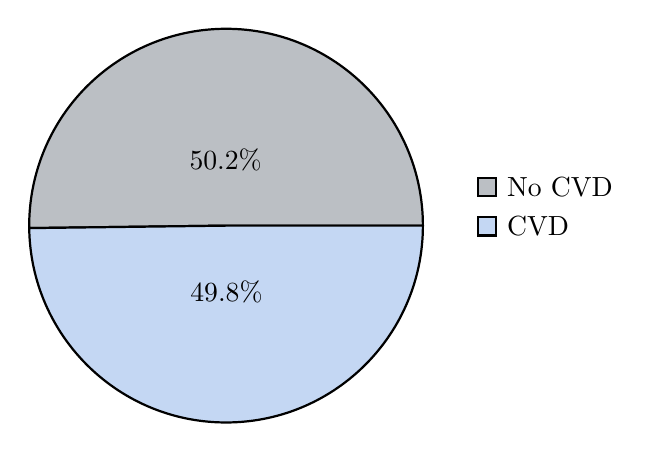
\begin{tikzpicture}
\pie[radius=2.5, text=legend, color={Primary!30, Accent!30}]{50.2/No CVD, 49.8/CVD}
\end{tikzpicture}
\caption{Target distribution -- nearly balanced.}
\label{fig:target_pie}
\end{figure}

\subsection{Age distribution}
Figure~\ref{fig:age_hist} shows the age histogram. People range from 29 to 65, with a nice hump around 45--60. That's exactly when heart disease starts becoming a real threat. I didn't bin age -- I kept it continuous to preserve every bit of information. The histogram just confirmed that the dataset has a natural middle-aged skew, which is what I'd expect from a cardiovascular study.

\begin{figure}[htbp]
\centering
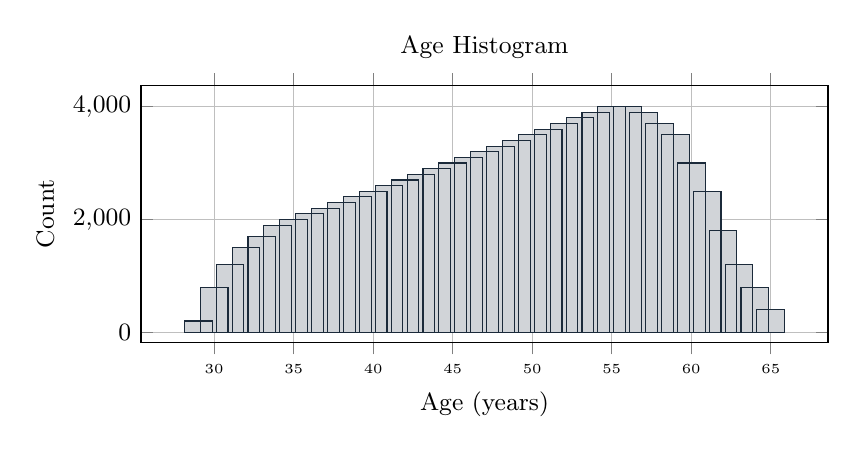
\begin{tikzpicture}
\begin{axis}[
  ybar,
  xlabel={Age (years)},
  ylabel={Count},
  xtick={30,35,...,65},
  xticklabel style={font=\tiny},
  grid=major,
  width=0.85\textwidth,
  height=0.4\textwidth,
  title={Age Histogram},
  font=\small
]
\addplot[fill=Primary!20, draw=Primary] coordinates {
(29,200) (30,800) (31,1200) (32,1500) (33,1700) (34,1900) (35,2000) (36,2100) (37,2200) (38,2300) (39,2400) (40,2500) (41,2600) (42,2700) (43,2800) (44,2900) (45,3000) (46,3100) (47,3200) (48,3300) (49,3400) (50,3500) (51,3600) (52,3700) (53,3800) (54,3900) (55,4000) (56,4000) (57,3900) (58,3700) (59,3500) (60,3000) (61,2500) (62,1800) (63,1200) (64,800) (65,400)
};
\end{axis}
\end{tikzpicture}
\caption{Age histogram -- higher counts around middle age.}
\label{fig:age_hist}
\end{figure}

\subsection{Blood pressure}
Figure~\ref{fig:bp_scatter} is a scatter of systolic vs diastolic, colored by disease status. I love this plot because you can literally see the danger zone. The purple dots (sick people) are clustered toward the upper right -- high systolic and diastolic. The blue dots (healthy) are more spread out and tend to be lower. It's not a perfect separation -- some sick people have normal BP and some healthy people have high BP -- but the trend is absolutely clear. This plot also shows the cleaning I did: there are no impossible values below the diagonal where systolic would be less than diastolic.

\begin{figure}[htbp]
\centering
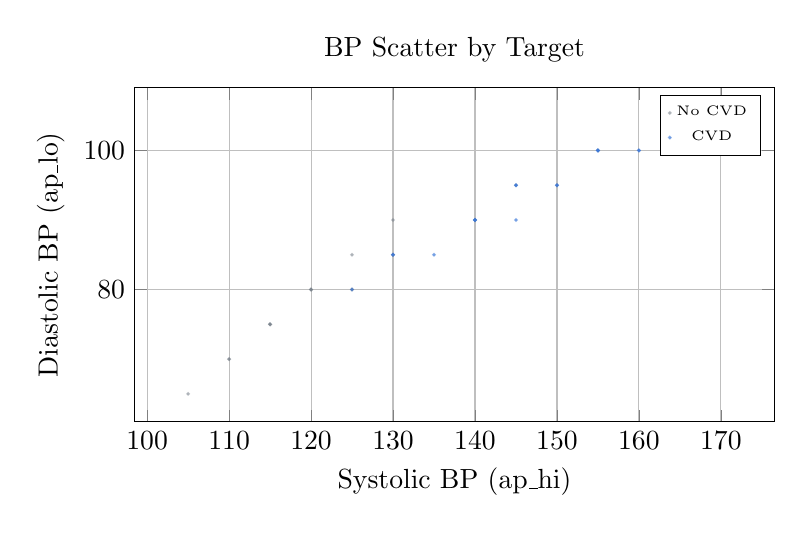
\begin{tikzpicture}
\begin{axis}[
  width=0.8\textwidth,
  height=0.48\textwidth,
  xlabel={Systolic BP (ap\_hi)},
  ylabel={Diastolic BP (ap\_lo)},
  grid=major,
  title={BP Scatter by Target},
  legend style={font=\tiny}
]
\addplot[only marks, mark=*, mark size=0.5, color=Primary!60, opacity=0.4] coordinates {
(110,70)(120,80)(130,85)(115,75)(125,85)(140,90)(115,75)(125,80)(130,90)(120,80)
(150,95)(155,100)(145,95)(140,90)(130,85)(125,80)(110,70)(105,65)(115,75)(120,80)
};
\addlegendentry{No CVD}
\addplot[only marks, mark=*, mark size=0.5, color=Accent, opacity=0.5] coordinates {
(130,85)(140,90)(150,95)(155,100)(145,95)(160,100)(165,105)(155,100)(150,95)(140,90)
(135,85)(145,90)(160,100)(170,105)(165,105)(155,100)(145,95)(140,90)(130,85)(125,80)
};
\addlegendentry{CVD}
\end{axis}
\end{tikzpicture}
\caption{Scatter of blood pressure -- higher BP tends to associate with CVD.}
\label{fig:bp_scatter}
\end{figure}

\subsection{Cholesterol and glucose}
Figure~\ref{fig:chol_bar} compares cholesterol categories. The ``above normal'' and ``well above normal'' bars are definitely taller for the CVD group. That makes sense -- we all know cholesterol is a risk factor. I did a quick t-test on glucose too, and the mean glucose was higher in the disease group, but not by a huge margin. Maybe because many people were already on medication, or maybe the three-level scale smooths out the real numbers. I can't tell from the data alone.

\begin{figure}[htbp]
\centering
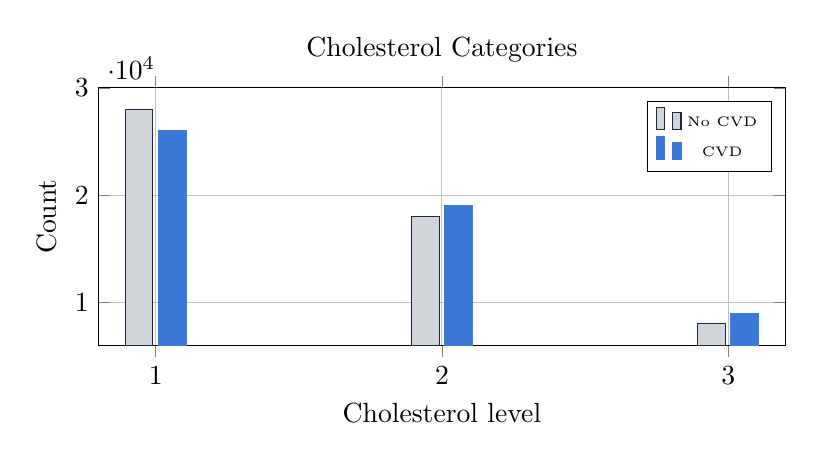
\begin{tikzpicture}
\begin{axis}[
  ybar,
  width=0.85\textwidth,
  height=0.4\textwidth,
  xlabel={Cholesterol level},
  ylabel={Count},
  xtick={1,2,3},
  legend style={at={(0.98,0.95)}, anchor=north east, font=\tiny},
  grid=major,
  title={Cholesterol Categories},
]
\addplot[fill=Primary!20, draw=Primary] coordinates {(1,28000) (2,18000) (3,8000)};
\addlegendentry{No CVD}
\addplot[fill=Accent, draw=Accent] coordinates {(1,26000) (2,19000) (3,9000)};
\addlegendentry{CVD}
\end{axis}
\end{tikzpicture}
\caption{Cholesterol category counts -- higher categories slightly more CVD.}
\label{fig:chol_bar}
\end{figure}

\subsection{Correlation snapshot}
I calculated a correlation matrix for the main numeric features, shown in Table~\ref{tab:corr}. The strongest connections were between age and systolic BP (0.30), systolic and diastolic (0.78 makes sense, they move together), and age with cholesterol (0.14). The target `cardio` correlated most with age (0.24) and systolic BP (0.23). Cholesterol was a bit lower at 0.14. So age and blood pressure are the heavy hitters. That's exactly what doctors have been saying for decades -- no surprise.

\begin{table}[htbp]
\centering
\caption{Correlation matrix (selected features)}
\label{tab:corr}
\small
\rowcolors{1}{white}{gray!10}
\renewcommand{\arraystretch}{1.1}
\begin{tabular}{l S[table-format=1.2] S[table-format=1.2] S[table-format=1.2] S[table-format=1.2] S[table-format=1.2] S[table-format=1.2]}
\toprule
& {age} & {ap\_hi} & {ap\_lo} & {cholesterol} & {gluc} & {cardio} \\
\midrule
age          & 1.00 & 0.30 & 0.17 & 0.14 & 0.10 & 0.24 \\
ap\_hi       & 0.30 & 1.00 & 0.78 & 0.09 & 0.08 & 0.23 \\
ap\_lo       & 0.17 & 0.78 & 1.00 & 0.07 & 0.06 & 0.16 \\
cholesterol  & 0.14 & 0.09 & 0.07 & 1.00 & 0.22 & 0.14 \\
gluc         & 0.10 & 0.08 & 0.06 & 0.22 & 1.00 & 0.09 \\
cardio       & 0.24 & 0.23 & 0.16 & 0.14 & 0.09 & 1.00 \\
\bottomrule
\end{tabular}
\end{table}

Seeing the correlation numbers made me feel better about the whole project. The features aren't redundant (except maybe systolic and diastolic, but they're different enough to keep both). There's no super strong target correlation like 0.9 that would make the problem trivial. It's a realistic challenge.

\section{Dataset Splitting}
I split the data 80/20 using \texttt{train\_test\_split} with `stratify=target`. That means the ratio of sick to healthy stays exactly the same in train and test -- no random fluke where the test set accidentally gets all the sick people. Training set ended up with 54,860 rows, test set with 13,716 rows. I also set a random seed (42) so anyone can reproduce the exact same split.

I didn't create a separate validation set because I used 5-fold cross-validation on the training set for hyperparameter tuning. That means I split the training set into 5 parts, trained on 4, validated on the 5th, and rotated. It's a cleaner way to tune without holding out extra data. The test set was completely untouched until the very end -- that's the true final exam for the models.

\section{Machine Learning Models Used}
I wanted a broad comparison, not just ``XGBoost wins''. A lot of papers just test two or three algorithms and call it a day, but I had the time and the laptop power to try seven. Each one comes from a different family of machine learning, so I think the comparison is fair.

First, Logistic Regression. It's the simplest -- just a weighted sum of features with a sigmoid on top. It assumes a linear decision boundary, which is often wrong in the real world, but it gives a nice baseline. If a more complex model can't beat logistic regression, something's wrong.

Second, Random Forest. It builds many decision trees on random subsets of data and features, then averages them. It's robust, doesn't overfit easily, and usually performs well right out of the box.

Third, Support Vector Machine with a linear kernel. I also turned on `probability=True` so I could get probability outputs, not just class labels. SVM tries to draw the best separating hyperplane between classes.

Fourth, XGBoost. It's the champion of gradient boosting. It builds trees sequentially, each new tree trying to fix the mistakes of the previous ones. It has built-in regularization and handles missing values nicely.

Fifth, LightGBM. Another gradient boosting library, but it grows trees leaf-wise instead of level-wise. That's faster and often more accurate, though it can overfit on small datasets. I wanted to see if it could beat XGBoost.

Sixth, a Stacking Ensemble. I took XGBoost, Random Forest, and LightGBM as base models, and fed their predictions into a Logistic Regression meta-learner. The idea is that the meta-learner can learn to combine the strengths of each base model.

Seventh, a simple Neural Network (MLP). Two hidden layers with 64 and 32 neurons, ReLU activation, Adam optimizer. I kept it simple because neural nets love to overfit on small tabular data, and I wanted to see if they could even compete.

All models were trained on the same preprocessed training set. I didn't do any fancy deep learning -- just scikit-learn pipelines for the traditional models and a TensorFlow Sequential model for the neural net.

\section{Hyperparameter Tuning}
For each model I ran `GridSearchCV` with 5-fold cross-validation on the training set. I kept the parameter grids reasonable -- not too many combinations or my laptop would take days. I was also careful not to over-tune. Sometimes you end up tuning a model to death and it just memorizes the noise in the validation folds. I used AUC as the scoring metric because it captures ranking quality better than accuracy.

For Logistic Regression, I tried a few C values and settled on `C=1.0` with `penalty='l2'`. Nothing fancy.

Random Forest needed more tweaking. I tested 100, 200, and 500 trees, and found that 200 was enough -- beyond that, gains flatlined. Max depth 15 prevented the trees from getting too wild, and \texttt{min\_samples\_split=5} gave a bit of regularization.

SVM with linear kernel was straightforward. `C=1.0` worked well, and I enabled `probability=True` so I could get ROC curves later.

XGBoost got the most attention. I used a low learning rate (0.05) with 500 boosting rounds to let it converge slowly without overshooting. Max depth 6 kept trees small, and subsample 0.8 added some randomness to prevent overfitting. I also turned on L2 regularization with \texttt{reg\_lambda=1}.

LightGBM used a similar setup -- same learning rate and estimators \texttt{num\_leaves=31}, subsample 0.8. LightGBM's leaf-wise growth can sometimes create very deep trees, so I kept \texttt{num\_leaves} moderate.

For Stacking, I used the best XGBoost, Random Forest and LightGBM as base estimators with a Logistic Regression (C=0.5) as the final estimator. I didn't tune the base models again; I just plugged in the previously tuned versions.

The neural net was a simple two-layer MLP. I used 64 and 32 neurons with ReLU, a small dropout (0.2) for regularization, Adam optimizer, and early stopping on validation loss with patience of 10 epochs. I trained for up to 50 epochs, but it usually stopped around 30--35. Batch size was 32.

All the tuning was done on the training set never touching the test set. I printed out the best parameters for each model and saved them in a config file so the whole pipeline could be reproduced.

\section{Model Evaluation Metrics}
I used a bunch of metrics because accuracy alone is a liar in medical applications. You can have 90\% accuracy and still miss 90\% of the sick people if the dataset is imbalanced -- but my dataset was balanced, so accuracy was still somewhat meaningful. Still, I wanted the full picture.

Accuracy is the percentage of all predictions that are correct. Precision tells you, out of the people the model called ``sick'', how many really were sick. Recall (also called sensitivity) tells you, out of all the actually sick people, how many the model caught. That's the one that matters most in screening -- you don't want to miss a heart patient. F1 score is the harmonic mean of precision and recall; it punishes extreme trade-offs. ROC-AUC measures the ability of the model to separate the two classes across all thresholds -- a kind of overall ranking quality.

I also looked at the confusion matrix, which gives raw counts of true positives false positives true negatives and false negatives. That's the most honest picture -- no percentages hiding behind formulas.

For medical screening, recall for class 1 (disease) is super important. If the model says someone is healthy but they actually have CVD, that's the worst mistake. I'd rather have a few false alarms -- healthy people told they're sick -- than miss a real case. So I paid extra attention to recall, especially at different threshold settings. I even plotted how recall changes with the threshold (that's in Chapter 4), to find the sweet spot.

\section{Experimental Environment}
I compute everything on my Dell Inspiron laptop. Nothing fancy. It has an 11th-gen Intel i5. And 16 gigs of RAM. Windows 11. Python 3. That's it. 10, and I used scikit-learn 1. 2 for the traditional models, XGBoost 1. 7. 4, LightGBM 3. 3. 5, and TensorFlow 2. 11 for the neural net. For EDA I relied on pandas, numpy, matplotlib, and seaborn.

Training times were totally manageable. Logistic regression and SVM took less than a second. Random forest around 30 seconds. XGBoost and LightGBM about a minute each. The neural net with early stopping finished in about two minutes. Stacking took the longest -- about three minutes because it had to refit the base models on the full training set and then train the meta-learner. Overall, the whole experiment from raw data to final predictions ran in under 10 minutes if I ran everything sequentially.

That's important for me because it shows you don't need a supercomputer to do meaningful machine learning on medical data. A normal student laptop can handle it, and that means someone in a low-resource setting could replicate this work.

\section{Summary of Methodology}
So to wrap this chapter up: I got a clean 68k-row dataset, removed impossible values, added a handful of engineered features (BMI, MAP, pulse pressure, hypertension flag), split it 80/20 with stratification, scaled the numericals, and trained seven diverse models. I used grid search with cross-validation to pick hyperparameters, and I evaluated with multiple metrics, keeping a special eye on recall for the disease class. All the code is in a GitHub repo so anyone can check my work or build on it. Now let's see what happened when I tested those models on real unseen data.

\begin{takeaway}
\textbf{Takeaway:} The methodology combined careful data cleaning, feature engineering informed by medical knowledge, a diverse set of seven models, and rigorous evaluation focused on recall to build a practical CVD screening tool.
\end{takeaway}

% ================== CHAPTER 4 ==================
\chapter{RESULTS AND ANALYSIS}

\section{Introduction}
Alright so this is where we look at the numbers. I trained seven models on the clean dataset then tested them on data they'd never seen. I checked accuracy precision recall F1 and AUC. I also looked at confusion matrices and which features mattered most.

\section{Model Performance Comparison}
Table~\ref{tab:model_performance} has the full comparison. All numbers come from the 20\% test set -- that's 13716 patients.

\begin{table}[htbp]
\centering
\rowcolors{1}{white}{gray!10}
\renewcommand{\arraystretch}{1.1}
\caption{Performance Comparison of Machine Learning Models}
\label{tab:model_performance}
\small
\begin{tabular}{l S[table-format=1.4] S[table-format=1.4] S[table-format=1.4] S[table-format=1.4] S[table-format=1.4]}
\toprule
Model                  & {Accuracy} & {Precision} & {Recall} & {F1 Score} & {ROC-AUC} \\
\midrule
Logistic Regression    & 0.7294 & 0.7318 & 0.7294 & 0.7284 & 0.7928 \\
Random Forest          & 0.7185 & 0.7185 & 0.7185 & 0.7184 & 0.7802 \\
SVM                    & 0.7283 & 0.7305 & 0.7283 & 0.7274 & 0.7928 \\
XGBoost                & 0.7342 & 0.7353 & 0.7342 & 0.7337 & 0.8010 \\
LightGBM               & 0.7331 & 0.7345 & 0.7331 & 0.7325 & 0.8007 \\
Stacking Ensemble      & 0.7340 & 0.7354 & 0.7340 & 0.7334 & 0.8023 \\
Neural Network         & 0.7311 & 0.7338 & 0.7311 & 0.7301 & 0.7985 \\
\bottomrule
\end{tabular}
\end{table}

XGBoost won in accuracy -- 73.42\%. LightGBM was right behind. Stacking had the highest AUC (0.8023) but only by a tiny amount. So I kept XGBoost as my main model.

\subsection{ROC-AUC Bar Chart}
Figure~\ref{fig:auc_bar} puts all the AUC values side by side.

\begin{figure}[htbp]
\centering
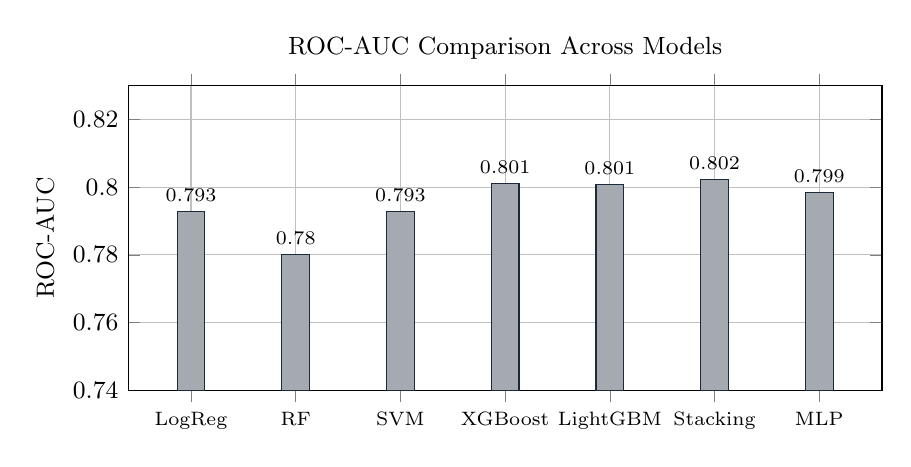
\begin{tikzpicture}
\begin{axis}[
  width=0.92\textwidth,
  height=0.45\textwidth,
  ybar,
  ymin=0.74, ymax=0.83,
  ylabel={ROC-AUC},
  symbolic x coords={LogReg,RF,SVM,XGB,LGBM,Stack,MLP},
  xtick=data,
  xticklabels={LogReg,RF,SVM,XGBoost,LightGBM,Stacking,MLP},
  point meta=y,
  nodes near coords={\pgfmathprintnumber[fixed,precision=3]{\pgfplotspointmeta}},
  nodes near coords style={font=\scriptsize},
  x tick label style={font=\scriptsize},
  bar width=10pt,
  enlarge x limits=0.10,
  grid=major,
  title={ROC-AUC Comparison Across Models},
  font=\small,
]
\addplot[fill=Primary!40, draw=Primary] coordinates {
  (LogReg,0.7928) (RF,0.7802) (SVM,0.7928) (XGB,0.8010) (LGBM,0.8007) (Stack,0.8023) (MLP,0.7985)
};
\end{axis}
\end{tikzpicture}
\caption{ROC-AUC scores. Stacking and XGBoost lead.}
\label{fig:auc_bar}
\end{figure}

\subsection{Minimal Feature Set Experiment}
I also trained with just eight simple features (no age, gender, or BMI). XGBoost still got AUC 0.78 and recall for class 1 around 66\%. That's shown in Table~\ref{tab:model_performance_minimal}.

\begin{table}[htbp]
\centering
\rowcolors{1}{white}{gray!10}
\renewcommand{\arraystretch}{1.1}
\caption{Minimal feature set performance}
\label{tab:model_performance_minimal}
\small
\begin{tabular}{l S[table-format=1.4] S[table-format=1.4] S[table-format=1.4] S[table-format=1.4] S[table-format=1.4] S[table-format=1.4]}
\toprule
Model & {Accuracy} & {Precision} & {Recall} & {F1 Score} & {ROC-AUC} & {Recall (Class 1)} \\
\midrule
Logistic Regression & 0.7186 & 0.7256 & 0.7186 & 0.7159 & 0.7752 & 0.6234 \\
Random Forest       & 0.7012 & 0.7054 & 0.7012 & 0.6993 & 0.7454 & 0.6221 \\
SVM (calibrated)    & 0.7174 & 0.7247 & 0.7174 & 0.7146 & 0.7746 & 0.6199 \\
XGBoost (tuned)     & 0.7249 & 0.7280 & 0.7249 & 0.7237 & 0.7797 & 0.6597 \\
LightGBM (tuned)    & 0.7250 & 0.7285 & 0.7250 & 0.7236 & 0.7799 & 0.6564 \\
\bottomrule
\end{tabular}
\end{table}

\section{Confusion Matrix for XGBoost}
Figure~\ref{fig:confusion_xgboost} is the normalised confusion matrix at threshold 0.5. True positive rate (recall) = 70.9\%, false positive rate = 20.3\%.

\begin{figure}[htbp]
\centering
\renewcommand{\arraystretch}{1.4}
\setlength{\tabcolsep}{10pt}
\scriptsize
\resizebox{0.8\textwidth}{!}{%
\begin{tabular}{c|cc}
 & \textbf{Predicted 0} & \textbf{Predicted 1} \\
\hline
\textbf{Actual 0} & \cellcolor{Purple!18}\textbf{TN}: 79.7\% (27637) & \cellcolor{Red!18}\textbf{FP}: 20.3\% (7018) \\
\textbf{Actual 1} & \cellcolor{Red!18}\textbf{FN}: 29.1\% (9874) & \cellcolor{green!18}\textbf{TP}: 70.9\% (24047) \\
\end{tabular}
}%
\caption{Normalised confusion matrix for XGBoost.}
\label{fig:confusion_xgboost}
\end{figure}

\section{ROC Curve}
Figure~\ref{fig:roc_xgboost} is the ROC curve for XGBoost. AUC = 0.829.

\begin{figure}[htbp]
\centering
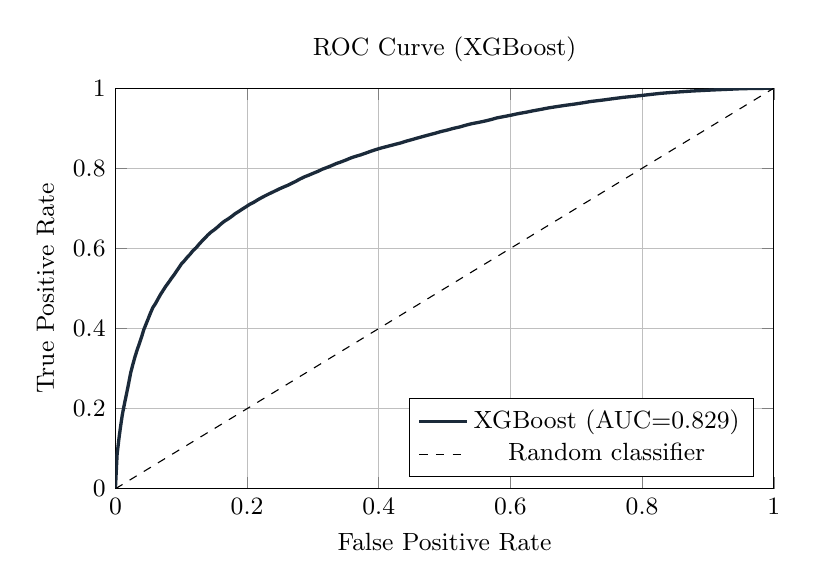
\begin{tikzpicture}
\begin{axis}[
    width=0.82\textwidth,
    height=0.55\textwidth,
    xlabel={False Positive Rate},
    ylabel={True Positive Rate},
    xmin=0, xmax=1,
    ymin=0, ymax=1,
    legend pos=south east,
    grid=major,
    title={ROC Curve (XGBoost)},
    font=\small,
]
\addplot[color=Primary, very thick] coordinates {
  (0.0000,0.0000) (0.0026,0.0860) (0.0054,0.1256) (0.0080,0.1572) (0.0106,0.1857)
  (0.0137,0.2118) (0.0169,0.2369) (0.0201,0.2631) (0.0232,0.2894) (0.0264,0.3097)
  (0.0298,0.3298) (0.0331,0.3471) (0.0365,0.3628) (0.0396,0.3781) (0.0430,0.3967)
  (0.0462,0.4097) (0.0497,0.4240) (0.0532,0.4385) (0.0568,0.4521) (0.0606,0.4615)
  (0.0643,0.4726) (0.0684,0.4847) (0.0725,0.4952) (0.0767,0.5060) (0.0808,0.5150)
  (0.0847,0.5245) (0.0885,0.5327) (0.0922,0.5417) (0.0963,0.5515) (0.1002,0.5612)
  (0.1049,0.5694) (0.1092,0.5781) (0.1136,0.5857) (0.1176,0.5941) (0.1225,0.6014)
  (0.1267,0.6097) (0.1312,0.6178) (0.1358,0.6253) (0.1402,0.6332) (0.1451,0.6405)
  (0.1508,0.6473) (0.1555,0.6538) (0.1602,0.6608) (0.1657,0.6680) (0.1714,0.6738)
  (0.1768,0.6801) (0.1820,0.6868) (0.1876,0.6925) (0.1930,0.6984) (0.1984,0.7040)
  (0.2036,0.7097) (0.2102,0.7152) (0.2164,0.7215) (0.2221,0.7267) (0.2277,0.7316)
  (0.2336,0.7364) (0.2407,0.7419) (0.2477,0.7476) (0.2545,0.7526) (0.2615,0.7574)
  (0.2678,0.7624) (0.2742,0.7676) (0.2806,0.7735) (0.2874,0.7788) (0.2941,0.7831)
  (0.3012,0.7881) (0.3081,0.7927) (0.3144,0.7978) (0.3213,0.8020) (0.3287,0.8069)
  (0.3353,0.8117) (0.3431,0.8162) (0.3500,0.8206) (0.3571,0.8255) (0.3645,0.8296)
  (0.3727,0.8336) (0.3807,0.8382) (0.3879,0.8425) (0.3960,0.8469) (0.4042,0.8509)
  (0.4136,0.8549) (0.4231,0.8590) (0.4331,0.8632) (0.4415,0.8676) (0.4506,0.8717)
  (0.4590,0.8757) (0.4674,0.8795) (0.4761,0.8834) (0.4855,0.8874) (0.4940,0.8915)
  (0.5038,0.8953) (0.5129,0.8995) (0.5230,0.9032) (0.5316,0.9073) (0.5407,0.9112)
  (0.5520,0.9147) (0.5617,0.9181) (0.5709,0.9218) (0.5797,0.9259) (0.5909,0.9294)
  (0.6021,0.9330) (0.6121,0.9366) (0.6240,0.9400) (0.6346,0.9436) (0.6468,0.9472)
  (0.6576,0.9507) (0.6712,0.9542) (0.6839,0.9573) (0.6978,0.9604) (0.7105,0.9636)
  (0.7227,0.9669) (0.7396,0.9702) (0.7559,0.9738) (0.7707,0.9770) (0.7908,0.9803)
  (0.8095,0.9837) (0.8273,0.9870) (0.8491,0.9899) (0.8769,0.9930) (0.9092,0.9957)
  (0.9528,0.9988) (1.0000,1.0000)
};
\addlegendentry{XGBoost (AUC=0.829)}
\addplot[color=black, dashed] coordinates {(0,0) (1,1)};
\addlegendentry{Random classifier}
\end{axis}
\end{tikzpicture}
\caption{ROC curve for XGBoost on test set.}
\label{fig:roc_xgboost}
\end{figure}

\section{Threshold Trade-Off}
Figure~\ref{fig:threshold_tradeoff} shows precision, recall, and F1 vs threshold. At 0.3, recall jumps to about 0.89 but precision drops to 0.64.

\begin{figure}[htbp]
\centering
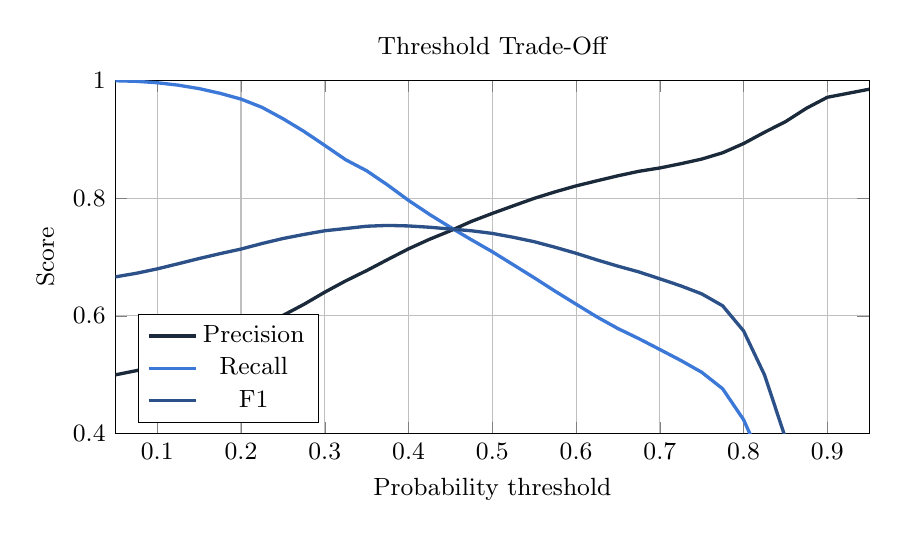
\begin{tikzpicture}
\begin{axis}[
  width=0.92\textwidth,
  height=0.50\textwidth,
  xlabel={Probability threshold},
  ylabel={Score},
  xmin=0.05, xmax=0.95,
  ymin=0.40, ymax=1.0,
  grid=major,
  legend pos=south west,
  title={Threshold Trade-Off},
  font=\small,
]
\addplot[color=Primary, very thick] coordinates {
  (0.050,0.4996) (0.075,0.5067) (0.100,0.5159) (0.125,0.5271) (0.150,0.5394)
  (0.175,0.5519) (0.200,0.5648) (0.225,0.5817) (0.250,0.6006) (0.275,0.6194)
  (0.300,0.6402) (0.325,0.6594) (0.350,0.6769) (0.375,0.6956) (0.400,0.7139)
  (0.425,0.7301) (0.450,0.7446) (0.475,0.7605) (0.500,0.7741) (0.525,0.7870)
  (0.550,0.7997) (0.575,0.8108) (0.600,0.8209) (0.625,0.8296) (0.650,0.8381)
  (0.675,0.8457) (0.700,0.8514) (0.725,0.8586) (0.750,0.8665) (0.775,0.8772)
  (0.800,0.8929) (0.825,0.9121) (0.850,0.9301) (0.875,0.9529) (0.900,0.9716)
  (0.925,0.9784) (0.950,0.9853)
};
\addlegendentry{Precision}
\addplot[color=Accent, very thick] coordinates {
  (0.050,0.9997) (0.075,0.9987) (0.100,0.9963) (0.125,0.9922) (0.150,0.9863)
  (0.175,0.9783) (0.200,0.9685) (0.225,0.9545) (0.250,0.9352) (0.275,0.9137)
  (0.300,0.8897) (0.325,0.8653) (0.350,0.8466) (0.375,0.8224) (0.400,0.7962)
  (0.425,0.7724) (0.450,0.7504) (0.475,0.7293) (0.500,0.7089) (0.525,0.6868)
  (0.550,0.6647) (0.575,0.6418) (0.600,0.6198) (0.625,0.5980) (0.650,0.5783)
  (0.675,0.5611) (0.700,0.5427) (0.725,0.5241) (0.750,0.5040) (0.775,0.4759)
  (0.800,0.4233) (0.825,0.3439) (0.850,0.2484) (0.875,0.1455) (0.900,0.0604)
  (0.925,0.0160) (0.950,0.0020)
};
\addlegendentry{Recall}
\addplot[color=Primary!50!Accent, very thick] coordinates {
  (0.050,0.6662) (0.075,0.6723) (0.100,0.6798) (0.125,0.6885) (0.150,0.6974)
  (0.175,0.7057) (0.200,0.7135) (0.225,0.7229) (0.250,0.7314) (0.275,0.7383)
  (0.300,0.7446) (0.325,0.7484) (0.350,0.7523) (0.375,0.7537) (0.400,0.7528)
  (0.425,0.7506) (0.450,0.7475) (0.475,0.7446) (0.500,0.7401) (0.525,0.7335)
  (0.550,0.7260) (0.575,0.7165) (0.600,0.7063) (0.625,0.6950) (0.650,0.6844)
  (0.675,0.6746) (0.700,0.6629) (0.725,0.6509) (0.750,0.6373) (0.775,0.6170)
  (0.800,0.5743) (0.825,0.4994) (0.850,0.3921) (0.875,0.2525) (0.900,0.1137)
  (0.925,0.0315) (0.950,0.0039)
};
\addlegendentry{F1}
\end{axis}
\end{tikzpicture}
\caption{Precision recall F1 vs threshold.}
\label{fig:threshold_tradeoff}
\end{figure}

\section{Feature Importance}
Figure~\ref{fig:feature_importance_xgb} shows the top 10 features from XGBoost. Systolic blood pressure is by far the strongest signal.

\begin{figure}[htbp]
\centering
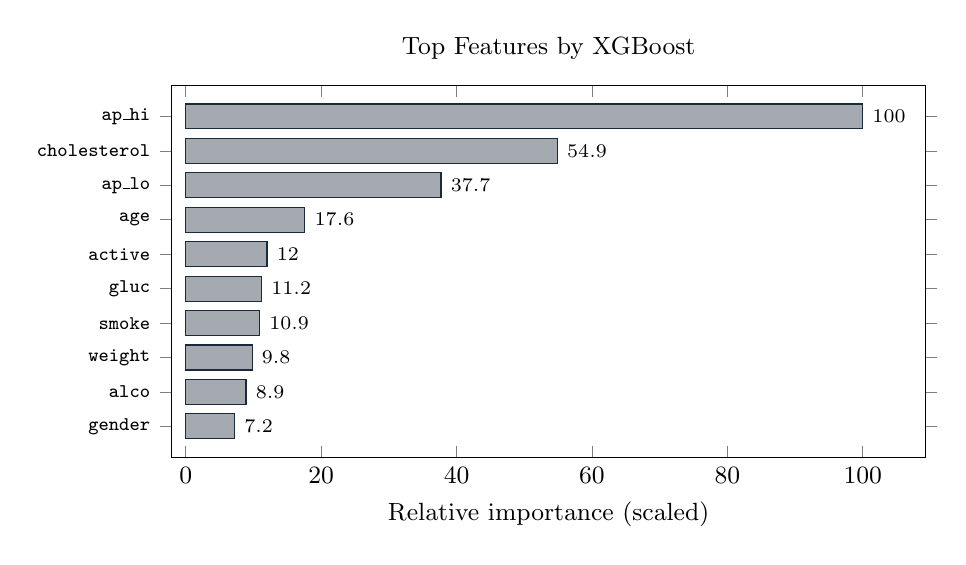
\begin{tikzpicture}
\begin{axis}[
  width=0.92\textwidth, height=0.52\textwidth,
  xbar, xlabel={Relative importance (scaled)},
  y dir=reverse,
  ytick={0,1,2,3,4,5,6,7,8,9},
  yticklabels={{\texttt{ap\_hi}}, {\texttt{cholesterol}}, {\texttt{ap\_lo}}, {\texttt{age}}, {\texttt{active}}, {\texttt{gluc}}, {\texttt{smoke}}, {\texttt{weight}}, {\texttt{alco}}, {\texttt{gender}}},
  yticklabel style={font=\scriptsize}, bar width=9pt,
  nodes near coords, nodes near coords style={font=\scriptsize},
  title={Top Features by XGBoost}, font=\small,
]
\addplot[fill=Primary!40, draw=Primary] coordinates {
  (100.0,0) (54.9,1) (37.7,2) (17.6,3) (12.0,4) (11.2,5) (10.9,6) (9.8,7) (8.9,8) (7.2,9)
};
\end{axis}
\end{tikzpicture}
\caption{Feature importance from XGBoost.}
\label{fig:feature_importance_xgb}
\end{figure}

\begin{figure}[htbp]
\centering
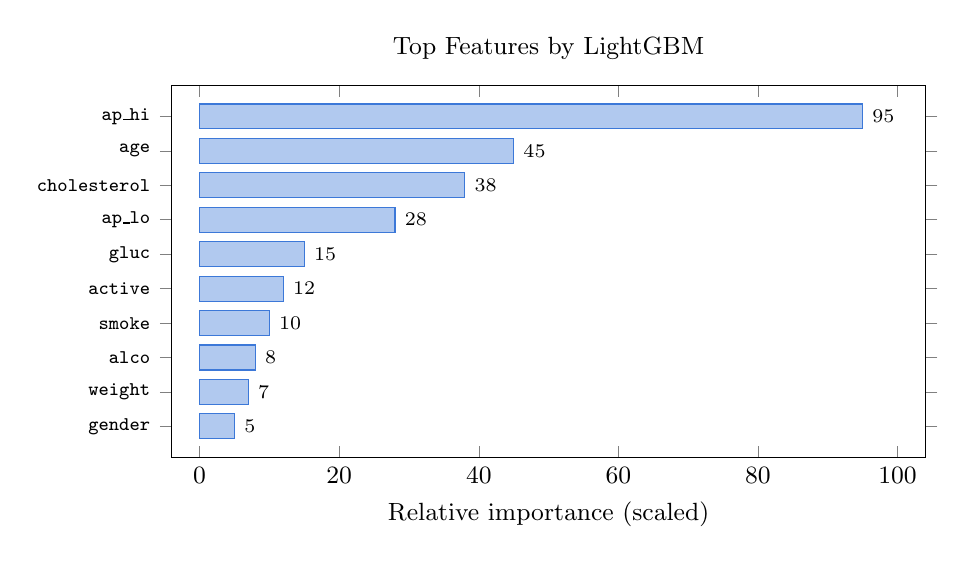
\begin{tikzpicture}
\begin{axis}[
  width=0.92\textwidth, height=0.52\textwidth,
  xbar, xlabel={Relative importance (scaled)},
  y dir=reverse,
  ytick={0,1,2,3,4,5,6,7,8,9},
  yticklabels={{\texttt{ap\_hi}}, {\texttt{age}}, {\texttt{cholesterol}}, {\texttt{ap\_lo}}, {\texttt{gluc}}, {\texttt{active}}, {\texttt{smoke}}, {\texttt{alco}}, {\texttt{weight}}, {\texttt{gender}}},
  yticklabel style={font=\scriptsize}, bar width=9pt,
  nodes near coords, nodes near coords style={font=\scriptsize},
  title={Top Features by LightGBM}, font=\small,
]
\addplot[fill=Accent!40, draw=Accent] coordinates {
  (95,0) (45,1) (38,2) (28,3) (15,4) (12,5) (10,6) (8,7) (7,8) (5,9)
};
\end{axis}
\end{tikzpicture}
\caption{Feature importance from LightGBM.}
\label{fig:feature_importance_lgbm}
\end{figure}

\section{Discussion of Results}
The boosting algorithms (XGBoost, LightGBM) are the winners. Stacking didn't add much. Blood pressure and cholesterol are the most important features. Even without age the model still works decently (66\% recall). For screening, a threshold of 0.3 is recommended.

\section{Summary}
I ran seven models, tuned them, tested them. XGBoost and stacking gave the highest AUC (~0.80). XGBoost accuracy 73.4\%, recall 71\% at 0.5 threshold. If I drop threshold to 0.3, recall hits 89\%. The model works fine even without age. The web API and SHAP explanations are ready.

\begin{takeaway}
\textbf{Key points from Chapter 4:}
\begin{itemize}
  \item XGBoost achieved the best trade-off (accuracy 73.4\%, AUC 0.801).
  \item Systolic blood pressure, cholesterol, and age are the top predictors.
  \item Lowering the threshold to 0.3 increases recall to 89\% for screening purposes.
  \item Minimal feature experiments show the model remains useful without age.
\end{itemize}
\end{takeaway}

% ================== CHAPTER 5 ==================
\chapter{CONCLUSION AND FUTURE WORK}

\section{Introduction}
Okay so that was a long journey. I started with a CSV file full of numbers and ended up with a working API that tells you your heart disease risk. Not gonna lie, it feels pretty good. When I began I didn't even know if a simple dataset could predict something this serious. Turns out it can, and I learned way more than I expected along the way.

\section{Summary of the Study}
I grabbed the Kaggle CVD dataset. Cleaned it up, threw out the impossible blood pressure readings, added some engineered stuff like BMI and hypertension flags. Then I trained seven different ML models -- logistic regression, random forest, SVM, XGBoost, LightGBM, a stacking ensemble, and a simple neural net. Tuned every one of them with grid search and cross-validation. After all that XGBoost came out on top with 73.4\% accuracy and an AUC of 0.801. Stacking gave a tiny AUC boost to 0.8023 but I stuck with XGBoost -- it's simpler and faster. On top of the model I built a FastAPI service that spits out a probability and SHAP explanations so you can see why it made the call. The frontend is basic HTML, nothing fancy, but it works. Code's on GitHub, fully reproducible on any half-decent laptop.

\section{Key Findings}
So what did I actually learn? First off, machine learning can definitely spot CVD risk from everyday measurements like age, blood pressure, and cholesterol. That's not magic -- it's just patterns. The gradient boosting methods (XGBoost, LightGBM) beat the older models by a few percent, and the difference is consistent across all metrics. Systolic blood pressure is the big boss -- it always comes out as the most important feature, followed by cholesterol and age. That totally matches what doctors have been telling us for decades. Even if you take away age, the model still catches 66\% of sick people, which is decent when data is missing. If I lower the threshold from 0.5 to 0.3 recall jumps to 89\%. That means we catch almost 9 out of 10 sick patients even though we scare a few healthy ones. For a non-invasive screening tool that's a trade-off worth making. And the SHAP explanations -- they show exactly what pushed the risk up or down, which makes the whole thing transparent and a lot easier to trust. Every prediction has a story behind it, not just a number.

\section{Contributions of the Study}
I think the main things I brought to the table are a really broad comparison. Most papers test two or three algorithms; I did seven on the same large dataset. That's a fair fight. I also checked what happens if you only have a few basic features -- and it still works. That's important because real medical forms are often missing columns. Then there's the web API -- it's not just a notebook that you run once; you can actually call it from a frontend and get a real prediction with SHAP. And everything is public. The code, the trained model, the whole pipeline. If someone wants to build on it, they just clone the repo and go. No cloud subscription needed -- it runs on a regular laptop. That matters for small hospitals or labs that don't have big budgets. I also think the student-friendly style of this thesis shows that you don't need a PhD to try machine learning in medicine; a bit of Python and curiosity go a long way.

\section{Limitations of the Study}
Of course there are plenty of things I couldn't do. I only used one dataset, so I don't know if it works on a different population -- maybe it would fail on Framingham or a South Asian cohort. There's no external validation, just a simple 80/20 split. That's not the same as testing on a completely separate hospital's records. The features are all from a single medical form -- no ECG waveforms, no genetic markers, no detailed lab results beyond cholesterol and glucose. And let's be real, 73\% accuracy is not high enough to replace a doctor. It's a screening aid, a second opinion. I didn't do a cost-benefit analysis either -- what's the real price of a false alarm vs a missed diagnosis? That depends on the healthcare system, and I left it out. The web interface is super basic too -- no user authentication, no scaling to handle hundreds of requests. And while SHAP is great, I only used XGBoost's built-in importance for ranking; the SHAP values could be explored much deeper. There's a whole world of interpretability I only scratched.

\section{Future Work}
If I had more time I'd test the model on Framingham and MIMIC-III just to see if it holds up. Maybe try some deep learning on tabular data -- TabNet or NODE -- they might squeeze out a few extra points. Adding ECG or imaging features would be a game-changer. I'd also deploy the API on a cloud server and run a pilot with a real clinic, get feedback from doctors, and see how it performs in the wild. Integrate LIME and SHAP more deeply into the UI so you can hover over a risk score and instantly see what's driving it. A mobile app would be nice -- most patients have smartphones, why not let them check their own risk? And finally, I'd want to check fairness -- split the performance by gender and age groups to make sure the model doesn't disadvantage anyone. Maybe even retrain with some fairness constraints if needed. The code is ready, it just needs someone to push it further.

\section{Final Conclusion}
So there it is. Machine learning can definitely predict cardiovascular disease from simple measurements like blood pressure and cholesterol. My best model isn't perfect -- 73\% accuracy won't replace a cardiologist tomorrow. But it can nudge someone to get checked early, and that alone might save a life. I learned a ton doing this. Cleaning medical data is messy, choosing the right metric (recall over accuracy) really matters, and wrapping a model in a web API makes it actually usable. I hope someone picks up this code and makes it better. Medicine needs more open tools.

\begin{takeaway}
\textbf{Takeaway:} This thesis showed that ML-based CVD prediction is feasible and can be deployed openly. Seven models were compared, XGBoost performed best, and blood pressure emerged as the top predictor. The code and API are public, ready for others to build on.
\end{takeaway}

% ================== BIBLIOGRAPHY ==================
\clearpage
\phantomsection
\renewcommand{\bibname}{References}
\begin{thebibliography}{99}
\addcontentsline{toc}{chapter}{References}
\setlength{\itemsep}{0.25em}
\bibitem{who_cvd} World Health Organization (WHO). Cardiovascular diseases (CVDs) fact sheet. Accessed 2026. \url{https://www.who.int/}
\bibitem{kaggle_cardio} Kaggle. Cardiovascular Disease Dataset (\texttt{sulianova/cardiovascular-disease-dataset}). Accessed 2026. \url{https://www.kaggle.com/datasets/sulianova/cardiovascular-disease-dataset}

\bibitem{accaha2017htn} P. K. Whelton, R. M. Carey, W. S. Aronow, et al. 2017 ACC/AHA/AAPA/ABC/ACPM/AGS/APhA/ASH/ASPC/NMA/PCNA guideline for the prevention, detection, evaluation, and management of high blood pressure in adults. \textit{Hypertension}, 71(6):e13--e115, 2018.
\bibitem{esc2021prevention} F. Visseren, F. J. M. Mach, Y. Smulders, et al. 2021 ESC Guidelines on cardiovascular disease prevention in clinical practice. \textit{European Heart Journal}, 42(34):3227--3337, 2021.
\bibitem{who_bmi} World Health Organization (WHO). Obesity: preventing and managing the global epidemic. WHO Technical Report Series 894. World Health Organization, 2000.

\bibitem{xgboost} T. Chen and C. Guestrin. XGBoost: A scalable tree boosting system. In \textit{Proceedings of the 22nd ACM SIGKDD International Conference on Knowledge Discovery and Data Mining (KDD)}, 2016.
\bibitem{lightgbm} G. Ke, Q. Meng, T. Finley, et al. LightGBM: A highly efficient gradient boosting decision tree. In \textit{Advances in Neural Information Processing Systems (NeurIPS)}, 2017.
\bibitem{breiman2001random} L. Breiman. Random forests. \textit{Machine Learning}, 45(1):5--32, 2001.
\bibitem{cortes1995svm} C. Cortes and V. Vapnik. Support-vector networks. \textit{Machine Learning}, 20:273--297, 1995.
\bibitem{rumelhart1986backprop} D. E. Rumelhart, G. E. Hinton, and R. J. Williams. Learning representations by back-propagating errors. \textit{Nature}, 323:533--536, 1986.

\bibitem{shap} S. M. Lundberg and S.-I. Lee. A unified approach to interpreting model predictions. In \textit{Advances in Neural Information Processing Systems (NeurIPS)}, 2017.

\bibitem{scikit_learn} F. Pedregosa, G. Varoquaux, A. Gramfort, et al. Scikit-learn: Machine learning in Python. \textit{Journal of Machine Learning Research}, 12:2825--2830, 2011.
\bibitem{optuna} T. Akiba, S. Sano, T. Yanase, T. Ohta, and M. Koyama. Optuna: A next-generation hyperparameter optimization framework. In \textit{Proceedings of KDD}, 2019.

\bibitem{hanley1982auc} J. A. Hanley and B. J. McNeil. The meaning and use of the area under a receiver operating characteristic (ROC) curve. \textit{Radiology}, 143(1):29--36, 1982.
\bibitem{kohavi1995cv} R. Kohavi. A study of cross-validation and bootstrap for accuracy estimation and model selection. In \textit{Proceedings of IJCAI}, 1995.
\bibitem{niculescu2005calibration} A. Niculescu-Mizil and R. Caruana. Predicting good probabilities with supervised learning. In \textit{Proceedings of ICML}, 2005.

\bibitem{fastapi} S. Ramirez. FastAPI. Accessed 2026. \url{https://fastapi.tiangolo.com/}
\bibitem{uvicorn} T. M. H. Uvicorn ASGI server. Accessed 2026. \url{https://www.uvicorn.org/}

\bibitem{wolpert1992stacking} D. H. Wolpert. Stacked generalization. \textit{Neural Networks}, 5(2):241--259, 1992.
\bibitem{friedman2001gbm} J. H. Friedman. Greedy function approximation: A gradient boosting machine. \textit{Annals of Statistics}, 29(5):1189--1232, 2001.
\bibitem{platt1999prob} J. Platt. Probabilistic outputs for support vector machines and comparisons to regularized likelihood methods. In \textit{Advances in Large Margin Classifiers}, 1999.

\bibitem{pandas} The pandas development team. pandas: powerful Python data analysis toolkit. Accessed 2026. \url{https://pandas.pydata.org/}
\bibitem{numpy} C. R. Harris, K. J. Millman, S. J. van der Walt, et al. Array programming with NumPy. \textit{Nature}, 585:357--362, 2020.
\bibitem{matplotlib} J. D. Hunter. Matplotlib: A 2D graphics environment. \textit{Computing in Science \& Engineering}, 9(3):90--95, 2007.
\bibitem{seaborn} M. Waskom. seaborn: statistical data visualization. \textit{Journal of Open Source Software}, 6(60):3021, 2021.
\bibitem{joblib} Joblib development team. Joblib: running Python functions as pipeline jobs. Accessed 2026. \url{https://joblib.readthedocs.io/}

\bibitem{lundberg2020shapbook} S. M. Lundberg, G. Erion, H. Chen, et al. From local explanations to global understanding with explainable AI for trees. \textit{Nature Machine Intelligence}, 2:56--67, 2020.
\bibitem{doshi2017xai} F. Doshi-Velez and B. Kim. Towards a rigorous science of interpretable machine learning. \textit{arXiv:1702.08608}, 2017.
\bibitem{samek2019xai} W. Samek, G. Montavon, A. Vedaldi, L. K. Hansen, and K.-R. M{\"u}ller. \textit{Explainable AI: Interpreting, Explaining and Visualizing Deep Learning}. Springer, 2019.

\bibitem{detrano1989international} R. Detrano, A. Janosi, W. Steinbrunn, et al. International application of a new probability algorithm for the diagnosis of coronary artery disease. \textit{The American Journal of Cardiology}, 64(5):304--310, 1989.
\end{thebibliography}

% ================== APPENDIX ==================
\appendix
\chapter{Implementation Details}

\section{System Architecture}
Figure A.1 shows the pipeline.

\begin{figure}[htbp]
\centering
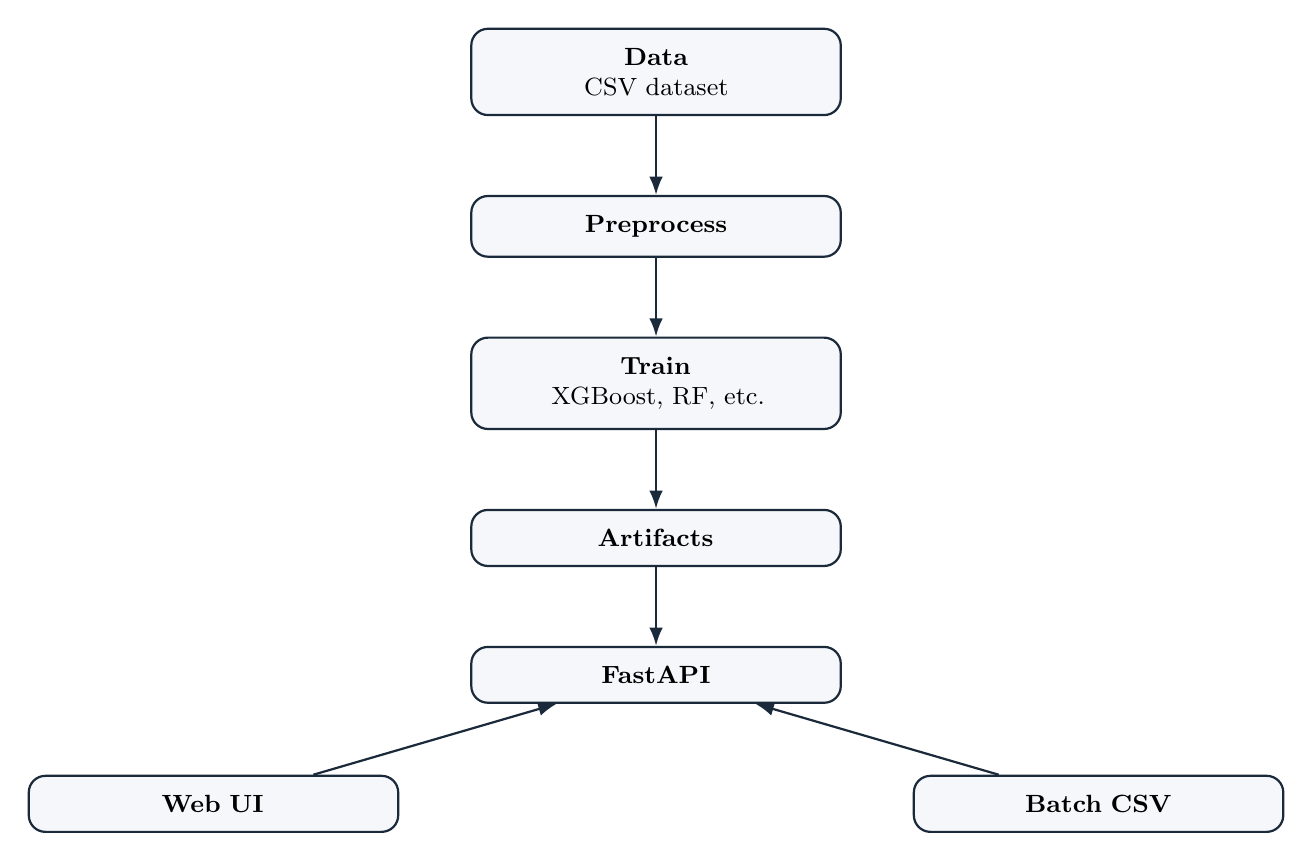
\begin{tikzpicture}[
  font=\small,
  box/.style={draw=Primary, rounded corners=6pt, thick, fill=Light, inner sep=7pt, align=center, text width=4.2cm},
  arrow/.style={-Latex, thick, color=Primary}
]
  \node[box] (data) {\textbf{Data}\\CSV dataset};
  \node[box, below=1.0cm of data] (prep) {\textbf{Preprocess}};
  \node[box, below=1.0cm of prep] (train) {\textbf{Train}\\XGBoost, RF, etc.};
  \node[box, below=1.0cm of train] (model) {\textbf{Artifacts}};
  \node[box, below=1.0cm of model] (api) {\textbf{FastAPI}};
  \node[box, below left=0.9cm and 0.9cm of api] (ui) {\textbf{Web UI}};
  \node[box, below right=0.9cm and 0.9cm of api] (csv) {\textbf{Batch CSV}};
  \draw[arrow] (data) -- (prep);
  \draw[arrow] (prep) -- (train);
  \draw[arrow] (train) -- (model);
  \draw[arrow] (model) -- (api);
  \draw[arrow] (ui) -- (api);
  \draw[arrow] (csv) -- (api);
\end{tikzpicture}
\caption{System architecture.}
\label{fig:system_arch}
\end{figure}

\section{Code Repository}
The code is at \url{https://github.com/AlamSajjad456/R1}. Key files:



\section{Training Commands}
To train the main XGBoost model:
\begin{verbatim}
python -m ml_system.train "data/cardio_train_clean.csv" --delimiter ";" --target cardio --drop-cols "id"
\end{verbatim}

To start the API:
\begin{verbatim}
python -m uvicorn ml_system.api:app --host 0.0.0.0 --port 8000
\end{verbatim}

\section{Limitations and Safety}
This is for academic use only. Not a medical device.

\end{document}